\documentclass{beamer}

\mode<presentation> {}
\usetheme{Madrid}

\makeatletter
\setbeamertemplate{footline}{%
  \leavevmode%
  \hbox{%
    \begin{beamercolorbox}[wd=.20\paperwidth,ht=2.25ex,dp=1ex,center]{author in head/foot}%
      \usebeamerfont{author in head/foot}\insertshortauthor
    \end{beamercolorbox}%
    \begin{beamercolorbox}[wd=.72\paperwidth,ht=2.25ex,dp=1ex,center]{title in head/foot}%
      \usebeamerfont{title in head/foot}\insertshorttitle
    \end{beamercolorbox}%
  }%
  \begin{beamercolorbox}[wd=.08\paperwidth,ht=2.25ex,dp=1ex,right]{date in head/foot}%
    \usebeamerfont{date in head/foot}%
    \usebeamertemplate{page number in head/foot}%
    \hspace*{2ex} 
  \end{beamercolorbox}
  \vskip0pt%
}
\makeatother
  
\usepackage{bbm}
\usepackage{apacite}
\usepackage{amssymb,amsthm,makeidx,verbatim,latexsym,amsfonts,graphicx,mathrsfs}
\usepackage{nomencl,tikz,caption,subcaption,enumitem,multicol,natbib,bm,lscape}
\usepackage{tasks,comment,url,float,pdfpages,tabularx,booktabs,longtable}
%\usepackage[hidelinks]{hyperref}
%\usepackage[tbtags]{amsmath}
\usepackage{colortbl,multirow,mathtools}
\usetikzlibrary{shapes.multipart}
\usetikzlibrary{positioning,calc,shapes.geometric,arrows,matrix,fit,backgrounds,intersections}

\setbeamertemplate{caption}[numbered] 


\DeclarePairedDelimiter\ceil{\lceil}{\rceil}
\DeclarePairedDelimiter\floor{\lfloor}{\rfloor}


\newcommand{\otoprule}{\midrule[\heavyrulewidth]}
\newcolumntype{A}{>{$}c <{$}}

\title[MACHINE LEARNING WITH APPLICATIONS IN AGRICULTURE]{MACHINE LEARNING WITH APPLICATIONS IN AGRICULTURE}

\author[ABIODUN ALLISON]{ABIODUN UTHMAN ALLISON} % Your name
\date[2021]{FEBRUARY, 2021}
\author[ABIODUN ALLISON]{\textbf{ABIODUN UTHMAN ALLISON \texorpdfstring{\\ MATRIC NO: 204603}{}}}
\institute{\textbf{A M.Sc. RESEARCH PROJECT SUBMITTED TO THE DEPARTMENT OF MATHEMATICS, FACULTY OF SCIENCE, UNIVERSITY OF IBADAN, IBADAN, NIGERIA.} \and \textbf{SUPERVISOR: PROF. G.O.S. EKHAGUERE}} 
 



\begin{document}

\begin{frame}
\titlepage % Print the title page as the first slide
\end{frame}

\begin{frame}
\frametitle{Overview} % Table of contents slide, comment this block out to remove it
\tableofcontents % Throughout your presentation, if you choose to use \section{} and \subsection{} commands, these will automatically be printed on this slide as an overview of your presentation
\end{frame}


\section{Introduction} % Sections can be created in order to organize your presentation into discrete blocks, all sections and subsections are automatically printed in the table of contents as an overview of the talk
%------------------------------------------------


\begin{frame}[allowframebreaks]
\frametitle{Introduction}
Agriculture could be referred to as the production, processing, promotion and distribution of agricultural products. It plays a critical role in the economy of developing countries. Besides supplying food and raw materials, agriculture also provides the populace with job opportunities. 

The Food and Agriculture Organization of the United Nations (FAO) estimates that pests and diseases lead to the loss of $20 - 40 \%$ of global food production, constituting a threat to food security (Food and Agriculture Organization of the United Nation, International Plant Protection Convention, 2017). 

Machine learning is the scientific study of algorithms and mathematical models that computer systems use to perform a specific task without using explicit instructions, relying on patterns and inference instead. It is a branch of Artificial Intelligence (AI) focused on the premise that, with minimal human interaction, systems can learn from data, recognize trends and make decisions. In supervised machine learning, a training set of $D$ input  vectors $\{\bm{x}_1, \bm{x}_2, \hdots , \bm{x}_D\}$ is used to tune the parameters of an adaptive model, along with their corresponding target vectors $\bm{y}$, in order to accurately predict vector $\hat{\bm{y}}$. We focus on a subset of supervised learning, called classification, where the aim is to assign each input vector to one of a finite number of discrete categories.

Computer vision, and object recognition in particular, has made tremendous advances in the past few years. In 2012, a large, deep convolutional neural network achieved a top-5 test error (the fraction of test images for which the correct label is not among the five labels considered most probable by the model) rate of $15.3\ \%$, at the Large Scale Visual Recognition Challenge (ILSVRC) 2012 image classification competition for the classification of $15$ million images into $22$ thousand possible categories {~\cite{Krizhevsky}}. 
\end{frame}

%------------------------------------------------
\section{Literature Review}
\begin{frame}[allowframebreaks]
\frametitle{Literature Review}
The idea of connecting units to local receptive fields on the input goes back to the perceptron in 1958 {~\cite{Rosenblatt58theperceptron}}. Although the perceptron initially seemed promising, the constraint that similar input patterns lead to similar outputs lead to an inability of the system to learn certain mappings from input to output, which proved that perceptrons could not be trained to recognise many classes of patterns. {~\cite{MinskyPapert:69}} pointed out that if we have the right connections from the input units to a large enough set of hidden units, we can always find a representation that will perform any mapping from input to output through these hidden units. LeNet-5, a pioneering 7-level convolutional network {~\cite{lecun-gradientbased-learning-applied-1998}} that classifies digits, was applied by several banks to recognize hand-written numbers on  cheques digitized in $32\times 32$ pixel images. This technique was constrained by the availability of computing resources since the ability to process higher resolution images requires larger and more layers of convolutional neural networks. With advancements in computing power driven by the advent of graphical processing units, convolutional neural networks were adopted more with great precision in the 2000s.
 
Different convolutional neural network (CNN) architectures has been applied in agriculture-analysis and phenotyping realm to solve complex problems. Measuring stalk count and stalk width of Sorghum plants {\cite{10.1007/978-3-319-67361-5_18}}; segmentation and counting of aphid nymphs {\cite{chen2018automatic}}; crop/weed segmentation {\cite{sa2018weedmap}}; plant disease detection and diagnosis {\cite{ferentinos2018deep}}; corn silage kernel processing {\cite{rasmussen2019maize}}; pod-counting and flower detection in soybean crop {\cite{zhang2019deep}}; classifying and counting insect pests in soybeans {\cite{tetila2019deep}};  detecting weeds in Bermuda grass {\cite{yu2019deep}}; extracting features of tea plant diseases from images {\cite{chen2019visual}}.
\end{frame}

%------------------------------------------------

\section{Logistic Regression}
\begin{frame}[allowframebreaks]
\frametitle{Logistic Regression}
Logistic regression is an algorithm for for binary classification - in which the goal is to learn a classifier that can input data  represented by feature vector $\bm{x} \in \mathbb{R}^{n_x}$ and present a label $y \in \{0,1\}$, where $n_x$ is the dimension of the vector $\bm{x}$. To transform the feature vector $\bm{x}$ into a scalar we input $\bm{x}$ to the linear predictive model with parameters, weight $\bm{w}\in \mathbb{R}^{n_x}$, and bias $b\in\mathbb{R}$
\begin{equation}\label{eqn:linear}
z = \bm{w}^T\bm{x} + b
\end{equation}
is used. The probabilistic sigmoid function $a=\sigma(z)=\dfrac{1}{1+e^{-z}}$  is then used to estimate the class of a new input. For a given vector $\bm{x}$, the prediction is estimated thus
\begin{equation} \label{eq:inference}
\text{Prediction} = \left\{
	\begin{array}{ll}
	0, & \text{if}\  a < 0.5 \\
    1, & \text{otherwise}
	\end{array} \right.
\end{equation}
Given feature vector $\bm{x}$, the aim is to output prediction $\hat{y}$:
\begin{equation}\label{eqn:t}
\hat{y} = P(y=1|\bm{x}) = a = \frac{1}{1+e^{-z}}
\end{equation}
To find optimal values for parameters $\bm{w}$ and $b$, we minimise the error function  which describes the error created by any arbitrary values of $\bm{w}$ and $b$. Since the predicted value belongs to either class $y=0$ or $y=1$, the output belongs to the Bernoulli distribution:
\begin{equation}\label{eqn:joint}
P(Y=y) = a^y(1-a)^{1-y}=\left\{\begin{array}{lcc}
						a & \text{if} & y=1 \\
						1-a & \text{if} & y=0
						\end{array}\right.
\end{equation}
Hence, we would to minimize the function $\mathrm{L}$ over $\bm{w}$ and $b$ 
\begin{equation}\label{eqn:loss}
\mathrm{L}(a,y) = -[y\log(a) + (1-y)\log(1-a)]
\end{equation}
$\mathrm{L}$ is the loss function which measures how good the output $a$ is when given the true label $y$ on a single training example $(\bm{x},y)$. 

Similarly, the overall loss function for the entire training set is given by 
\begin{equation}\label{eqn:cost}
\begin{split}
\mathrm{J}(\bm{w}, b) &=-\frac{1}{m} \sum_{i=1}^{m}\left[\left(y^{(i)} \log \left(a^{(i)}\right)+\left(1-y^{(i)}\right) \log \left(1-a^{(i)}\right)\right]\right. \\
	&=\frac{1}{m} \sum_{i=1}^{m} \mathrm{L}\left(a^{(i)}, y^{(i)}\right)
\end{split}
\end{equation}
Equation \eqref{eqn:cost} is called the {cost function} which measures how well parameters $\bm{w}$ and $b$ are doing on the entire training set $(\bm{X},\bm{y})$. A global minimum is guaranteed since $\mathrm{J}(\bm{w}, b)$ is convex.
\end{frame}

\begin{frame}[allowframebreaks]
\frametitle{Gradient Descent}
To find the parameters $\bm{w},\;b$ that minimizes the cost function $\mathrm{J}(\bm{w},\;b)$, we use the gradient descent algorithm; which is an optimisation algorithm used to minimize some function by iteratively moving in the direction of steepest descent as defined by the negative of the gradient. Choosing a suitable learning rate $\alpha > 0$, at time step $k$ gradient descent performs the iterative method:
\begin{equation}\label{eqn:gd}
\bm{x}^{k+1} = \bm{x}^k - \alpha \nabla f(\bm{x}^k)
\end{equation}
where $f:\mathbb{R}^n \rightarrow \mathbb{R}$ is the objective function to be minimised, and $\bm{x} \in \mathbb{R}^n$
\begin{theorem}[\cite{bottou2018optimization}]
Suppose the function $f: \mathbb{R}^{n} \rightarrow \mathbb{R}$ is convex and twice continuously differentiable, and it is L-smooth (i.e. its gradient is Lipschitz continuous with constant $L>0$): 
\begin{equation}\label{eqn:lipschitz}
\|\nabla f(\bm{x})-\nabla f(\bm{y})\|_{2} \leq L\|\bm{x}-\bm{y}\|_{2}
\end{equation}
for any $\bm{x}, \bm{y}\in \mathbb{R}^m$. Gradient descent for $k$ iterations with  fixed learning rate $\alpha \leq 1 / L$  satisfies
\begin{equation}\label{eqn:sublinear_conv}
f\left(\bm{x}^{(k)}\right)-f\left(\bm{x}^{*}\right) \leq \frac{\left\|\bm{x}^{(0)}-\bm{x}^{*}\right\|_{2}^{2}}{2 \alpha k}
\end{equation}
where $f\left(\bm{x}^{*}\right)$ is the optimal value of $f(\bm{x})$. 
\end{theorem}
Intuitively, this means that gradient descent converges sublinearly with rate $\mathcal{O}(1 / k)$.

Using, gradient descent, the computing cost for each independent variable iteration grows linearly with the dataset size. Therefore, when the model training data instance is large, the cost of gradient descent for each iteration will be very high.

Stochastic gradient descent (SGD) reduces computational cost at each iteration by uniform sampling an index $i_k \in\{1, \ldots, m\}$ for data instances at random, and compute the gradient $\nabla f_{i_{k}}(\bm{x})$ to update $\bm{x}$:
\begin{equation}\label{eqn:sgd}
\bm{x}^{k+1}=\bm{x}^{k}- \alpha_k \cdot \nabla f_{i_{k}}\left(\bm{x}^{k}\right), \quad k=1,2,3, \ldots
\end{equation}
where $i_{k} \in\{1, \ldots, m\}$ is some chosen index at iteration $k$ and $\alpha_k$ is the learning rate at iteration $k$. Stochastic gradient descent uses an unbiased estimate of the gradient $\nabla f(\bm{x})$ at each step, i.e,
\begin{equation}\label{eqn:sgd_est}
\mathbb{E}[\nabla f_{i_{k}}(\bm{x})]=\frac{1}{m} \sum_{i=1}^{m} \nabla f_{i}(\bm{x})  = \nabla f(\bm{x})
\end{equation}

A popular method used in machine learning is to compute the gradient against more than one training example, called a minibatch, at each step. This method improves computational efficiency compared to stochastic gradient descent, because the gradient can be calculated using vectorisation libraries rather than computing each step separately. In minibatch stochastic gradient descent,  we choose a random subset $I_{k} \subseteq\{1, \ldots, m\},\;\left|I_{k}\right|=b \ll m,$ repeat:
\begin{equation}\label{eqn:mini_sgd}
\bm{x}^{k+1}=\bm{x}^{k}- \alpha_k \cdot \frac{1}{b} \sum_{i \in I_{k}} \nabla f_{i}\left(\bm{x}^{k}\right), \quad k=1,2,3, \ldots
\end{equation}
\end{frame}

\begin{frame}
\frametitle{Regularisation}
Regularisation is used to prevent a model from overfitting - where the model would memorise the data and perform poorly on the hold out test data. It involves modulating the amount of information the model can store by reducing the number of learnable parameters in the model. Regularization is done by adding to the cost function of the model a cost associated with having large weights. With $L^2$ regularisation, the cost added is the square $L^2$ norm of the weights: 
\begin{equation}\label{eqn:cost_regularisation}
\mathrm{J}(\bm{w}, b) =-\frac{1}{m} \sum_{i=1}^{m}\left[\left(y^{(i)} \log \left(a^{(i)}\right)+\left(1-y^{(i)}\right) \log \left(1-a^{(i)}\right)\right]\right. + \frac{\lambda}{2}\|\bm{w}\|_2^2
\end{equation}
where $\lambda\geq 0$ is an hyperparameter called the regularisation constant, and it governs the amount of regularisation.
\end{frame}

\section{Neural Networks}
\begin{frame}[allowframebreaks]
\frametitle{Neural Networks}
Logistic regression and similar vanilla machine learning models discussed earlier only work effectively in cases where a hyperplane can distinguish the line between class $y=0$ and class $y=1$. But there are situations in which the data are not well separated by a linear classifier, neural networks are ideal to solve these problems.

A basic neural network model  can be described a series of functional transformations. First we construct linear combinations of the input variables $[\bm{x}_1,\bm{x}_2,\hdots,\bm{x}_D]$ in the form
\begin{equation}\label{z1}
\bm{z}^{[1]} = \bm{W}^{[1]}\bm{x} + \bm{b}^{[1]}
\end{equation}
the superscript $[1]$ indicates that the corresponding parameters $\bm{W}$ (weights) and $\bm{b}$ (biases) are in the first `layer' of the network. Each of the linear combinations is then transformed using a differentiable, non-linear activation function $g(.)$ to give
\begin{equation}\label{a1}
\bm{a}^{[1]} = g^{[1]}(\bm{z}^{[1]})
\end{equation}
where $\bm{a}^{[l]}$ represents the activations at layer $l$. These quantities in the context of neural networks, are called hidden units which forms the hidden layer. These values are again linearly combined to give output unit activations
\begin{equation}\label{z2}
\bm{z}^{[2]} = \bm{W}^{[2]}\bm{a}^{[1]} + \bm{b}^{[2]}
\end{equation}
This transformation corresponds to the second layer of the network. Finally, the output unit activations are transformed using an appropriate activation function to give a set of network output $\hat{y}$. The choice of activation function is determined by the nature of the data and the assumed distribution of target variables. 
\begin{figure}[H]
\def\layersep{3.5cm}
\tiny
\centering
%\begin{subfigure}{.5\textwidth}
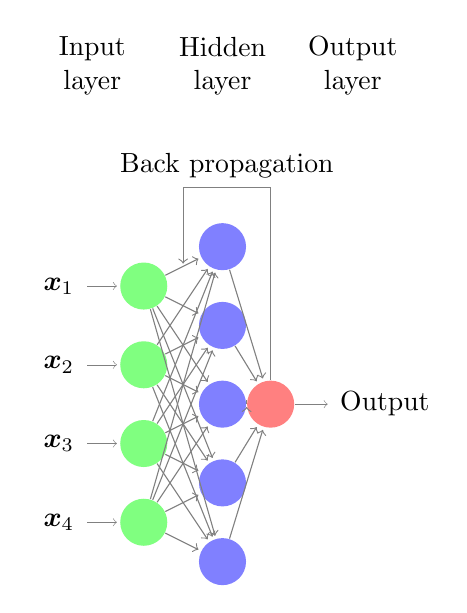
\begin{tikzpicture}[%
  shorten >=1pt,->,draw=black!50, node distance=\layersep,
  %every pin edge={<-,shorten <=1pt},
  neuron/.style={circle,fill=black!25,minimum size=17pt,inner sep=0pt},
  input neuron/.style={neuron, fill=green!50},
  output neuron/.style={neuron, fill=red!50},
  hidden neuron/.style={neuron, fill=blue!50},
  annot/.style = {text width=4em, text centered}
  ]
  % Draw the input layer nodes
  \foreach \name / \y in {1,...,4}
  % This is the same as writing \foreach \name / \y in {1/1,2/2,3/3,4/4}
  \node[input neuron, pin={[pin edge={<-,shorten <=1pt}]left: $\bm{x}_\y$}] (I-\name) at (0,-\y) {};

  % Draw the hidden layer nodes
  \foreach \name / \y in {1,...,5}
  \node[hidden neuron] (H-\name) at (\layersep,-\y cm+0.5cm) {};

  % Draw the output layer node
  \node[output neuron,pin={[pin edge={->}]right:Output}, right=of H-3] (O) {};

  % Connect every node in the input layer with every node in the
  % hidden layer.
  \foreach \source in {1,...,4}
  \foreach \dest in {1,...,5}
  \path (I-\source) edge (H-\dest);

  % Connect every node in the hidden layer with the output layer
  \foreach \source in {1,...,5}
  \path (H-\source) edge (O);

  % Annotate the layers
  \node[annot,above=15mm of H-1] (hl) {Hidden layer};
  \node[annot,left=of hl] {Input layer};
  \node[annot,right=of hl] {Output layer};
  %%% 
  \coordinate (H-I-1) at ($(H-1)!0.5!(I-1)$);
  \draw (O) |- ($(H-I-1) +(0,1)$) node[above,pos=0.75]{Back propagation} -- (H-I-1);
\end{tikzpicture}
\caption{Network diagram for one hidden layer neural network}
\label{fig:hidden}
\end{figure} 
Let $n^{[i]}$ be the number of nodes at layer $i$. The dimension of the parameters $\bm{W}^{[1]}$, $\bm{b}^{[1]}$, $\bm{W}^{[2]}$ and $\bm{b}^{[2]}$ depends on $n^{[i]}$ at different layers. The dimensions are 
\begin{multicols}{2}
\begin{itemize}[label=-]
\item $\bm{W}^{[1]}$ - $(n^{[1]},n^{[0]})$
\item $\bm{W}^{[2]}$ - $(n^{[2]},n^{[1]})$
\item $\bm{b}^{[1]}$ - $(n^{[1]},1)$
\item $\bm{b}^{[2]}$ - $(n^{[2]},1)$
\end{itemize}
\end{multicols}
The mostly widely used activation function in hidden layers is the Rectified Linear Activation Function (ReLU), it  is a simple calculation that returns the value provided as input directly, or the value $0$ if the input is $0$ or negative. The function is given by:
\begin{equation}\label{eqn:relu}
h(z) = \max(0,z)
\end{equation}
\begin{figure}[H]
\centering 
\includegraphics[scale=0.5]{png/relu.png} 
\caption{ReLU function}
\label{fig:relu}
\end{figure}
Softmax function is widely used as the activation function of the output layer for classification classes with more than two classes. it would squeeze the outputs for each class between $0$ and $1$ and would also divide by the sum of the outputs. This essentially gives the probability of the input being in a particular class. The standard (unit) softmax function $\sigma :\mathbb{R}^{K}\to \mathbb{R}^{K}$ is defined by the formula:
\begin{equation}\label{eqn:softmax}
\sigma (\bm{z} )_{i}={\frac {e^{z_{i}}}{\sum _{j=1}^{K}e^{z_{j}}}}{\text{ for }}i=1,\dotsc ,K{\text{ and }}\bm{z} =(z_{1},\dotsc ,z_{K})\in \mathbb {R} ^{K}
\end{equation}
After applying softmax, each component would be in the interval $(0,1)$, and the components will add up to $1$, so that they can be interpreted as probabilities. Furthermore, the larger input components will correspond to larger probabilities.
\end{frame}

\begin{frame}
\frametitle{Backpropagation}
Neural networks are trained using backpropagation. Backpropagation refers to the method of calculating the gradient of neural network parameters using  chain rule. The core insight is that the objective function derivative with respect to a module's input can be computed by working backwards from the gradient with respect to that module's output (or the corresponding module's input). The backpropagation equation can be repeatedly applied to propagate gradients through all modules, starting from the output at the top (where the network produces its prediction) all the way down (where the external input is fed). 
\end{frame}

\section{Convolutional Neural Networks}
\begin{frame}[allowframebreaks]
\frametitle{Convolutional Layers}
Convolutional neural networks (CNNs) are similar to neural networks in that they consist of neurons which optimize themselves through learning, each neuron will still receive an input and perform an operation such as a scalar product followed by a non-linear function. They are designed to process data that are in form of multiple arrays, such as a color image consisting of three 2D arrays containing pixel intensities in three color channels; red, green and blue (RGB). CNNs are mostly made up of stacks convolutional layers followed by non-linearity layers, then pooling layers and fully connected layers with softmax at the output layer.

In a convolutional layer, an input array and a convolution kernel array are combined to produce an array through a cross-correlation operation, a scalar bias is added to the array to produce an output, followed by a non-linear activation function (mostly ReLU) being applied to the output array. 

Cross-correlation is the measure of the overlap between two functions $f,g:\mathbb{R}^n
 \rightarrow \mathbb{R}$ when one of the functions is shifted by $\bm{x}$, it is given by
\begin{equation}\label{eqn:2d_cross}
(\bm{I} \star \bm{K}) (i,j) = \sum_m \sum_n \bm{I}(i+m,j+n) \bm{K}(m,n)
\end{equation} 
In a two-dimensional cross-correlation operation, a convolutional kernel (or filter) is positioned at the at the top-left corner of the input array and we slide it across the input array, both from left to right and top to bottom. When the kernel slides to a certain position, the input subarray contained in that position and the kernel array are multiplied elementwise and the resulting array is summed up yielding a single scalar value. This result if precisely the value of the output array at the corresponding location. Since the kernel has a width greater than one, and we can only compute the cross-correlation for locations where the kernel fits wholly within the image, the output size is given by the input size $H \times W$ minus the size of the convolutional kernel $h \times w$ via $(H - h + 1) \times (W - w + 1)$, since we need enough space to shift the convolutional kernel across the image.

Convolution layers are also useful for local feature detection, since a feature that is useful in one part of the image is probably useful in another part of the image.
\begin{figure}[H]
\centering
\includegraphics[scale=0.5]{png/cross_corr_2_dim.png}
\caption{Cross-correlation computation with $2$ input channels, {\cite{zhang2020dive}}}
\label{fig:2-dim}
\end{figure} 
\end{frame}



\begin{frame}[allowframebreaks]
\frametitle{Padding and Stride}
Since kernels generally have width and height greater than $1$, after applying many successive convolutions, we tend to wind up with outputs that are considerably smaller than our input. To keep the shape of the input, we add additional filler pixels around the boundary of our input image, thereby increasing the image's effective size. Typically, we set the values of the extra pixels to zero.
\begin{figure}[H]
\centering
\includegraphics[scale=0.5]{png/padding.png}
\caption{Two-dimensional cross-correlation with padding, {\cite{zhang2020dive}}}
\label{fig:pad}
\end{figure}
When computing the cross-correlation, we begin with the convolution window at the top-left corner of the input tensor, and then slide it both down and to the right over all locations, defaulting to sliding one element at a time in previous examples. However, often we shift our window more than one element at a time, skipping the intermediate positions, either for computational effectiveness or because we want to downsample. We refer to the number of rows and columns traversed per slide as the stride. In practice, we apply the same amount of stride vertically and horizontally. Hence, given an input image with size $H \times H$, a convolution kernel with size $h \times h$, applied at stride $s$ with pad $p$, the output would be of height and width
\begin{equation}\label{eqn:pad_stride}
\floor*{\dfrac{H + 2p - h}{s} + 1}
\end{equation}
\end{frame}


\begin{frame}[allowframebreaks]
\frametitle{Pooling Layers}
Like convolutional layers, pooling operators consist of a fixed-shaped window that slides across all regions of the input according to its stride, computing a single output for each position crossed by the window. Pooling layers serves the dual purpose of merging semantically similar features into one and of spatially downsampling representations. However, unlike the cross-correlation operation of inputs and kernels in the convolutional layer, the pooling layer does not include any parameters, i.e., there is no kernel. Instead, pooling operators are deterministic, usually measuring either the maximum (max pooling) or the average value (average pooling) of the elements in the pooling window. 
\begin{figure}[H]
\centering
\includegraphics[scale=0.7]{png/pooling.png}
\caption{Maximum pooling with a pooling window shape of $2 \times 2$, {\cite{zhang2020dive}}}
\label{fig:pool}
\end{figure}
\end{frame}


\begin{frame}[allowframebreaks]
\frametitle{Adam Optimiser}
We introduced minibatch  gradient descent earlier, which improved on the convergence rate of gradient descent, where we made parameter updates using a minibatch with size $b$, instead of the whole dataset at each iteration. In practice, common loss functions for neural networks are highly non-convex, minimising the loss becomes a challenge using SGD algorithms due to saddle points in the function {\cite{dauphin17e}}, saddle points are usually surrounded by a plateau of the same error, which makes it notoriously difficult for gradient descent to escape, as the gradient is close to zero in all dimensions. Momentum {\cite{qian1999momentum}} is a method that helps speed gradient descent in the relevant direction and dampens oscillations, by adding a fraction $\rho$ of the update vector of the previous time step to the current update vector. 

Adaptive Moment Estimation (Adam) {\cite{kingma2014adam}} computes individual adaptive learning rates for different parameters from estimate of the first and second moments of the gradients. Adam stores an exponentially decaying average of past squared gradients $\bm{v}^k$, and an exponentially decaying average of past gradients $\bm{m}^k$, similar to momentum. The decaying averages of past and past squared gradients $\bm{m}^k$ and $\bm{v}^k$ respectively are calculated as follows:
\begin{equation}\label{eqn:adam_mean}
\begin{array}{l}
\bm{m}^k = \beta_1\bm{m}^{k-1} + (1-\beta_1)\bm{g}^k \\
\bm{v}^k = \beta_2\bm{v}^{k-1} + (1-\beta_2)(\bm{g}^k)^2
\end{array}
\end{equation} 
$\bm{m}^k$ and $\bm{v}^k$ are estimates of the first moment (the mean) and the second moment (the uncentered variance) of the gradients respectively. Since $\bm{m}^k$ and $\bm{v}^k$ are initialized as vectors of $0$'s, they become biased towards zero, especially during the initial time steps, and especially when the decay rates are small, i.e., $\beta_1$ and $\beta_2$are close to 1). Bias-corrected first and second moment estimates are calculated to tackle this problem:
\begin{equation}\label{eqn:adam_bias}
\begin{array}{l}
\hat{\bm{m}}^k = \dfrac{\bm{m}^k}{1-\beta^k_1} \\
\hat{\bm{v}}^k = \dfrac{\bm{v}^k}{1-\beta^k_2}
\end{array}
\end{equation}
The Adam update rule is given as:
\begin{equation}\label{eqn:adam}
\bm{x}^{k+1} = \bm{x}^{k} - \dfrac{\alpha}{\sqrt{\hat{\bm{v}}^k} + \epsilon}\; \hat{\bm{m}}^k
\end{equation}
Adam works well in practice and compares favourably to other adaptive learning-method algorithms.
\end{frame}

\begin{frame}[allowframebreaks]
\frametitle{Transfer Learning}
To improve training accuracy and speed up training time we adopt transfer learning. Transfer learning can be described as the improvement of learning of a new task by the transition of information from a previously learned similar task, model weights from pre-trained models created for large-scale image-classification datasets, such as ImageNet are reused to solve similar image-classification tasks. VGG16 and ResNext-50 were used as the pre-trained models in this project.
\end{frame}

\begin{frame}[allowframebreaks]
\frametitle{VGG16}
VGG16  made  improvement over AlexNet {~\cite{Krizhevsky}} by replacing large kernel-sized filters ($11$ and $5$ in the first and second convolutional layer respectively) with stacks of $3 \times 3$ kernel-sized filters. Each stack of  $3 \times 3$ convolutional layer with stride $1$, pad $1$ and different depths is followed by $2 \times 2$ max pooling layers applied at stride $2$, three fully-connected (FC) layers follow the final max pool layer; the first two have 4096 channels each, the third performs 1000-way ILSVRC classification and thus contains 1000 channels (one for each class), the final layer is the softmax layer and ReLU is applied to all hidden layers (Figure \ref{fig:vgg16_arch}). It was shown that the added depth and smaller filters is beneficial for classification accuracy.

\begin{figure}[H]
\centering
\includegraphics[scale=0.5]{png/vgg16.png}
\caption[VGG16 model architecture]{VGG16 model architecture, \protect{\cite{Das2019DoubleCV}}}	
\label{fig:vgg16_arch}
\end{figure} 
\end{frame}

\begin{frame}[allowframebreaks]
\frametitle{ResNext}
Deep networks are susceptible to vanishing/exploding gradients, making it harder to optimise compared to shallow networks. During backpropagation, deriving partial derivative of the error function with respect to the current weight in each iteration of training, has the effect of multiplying $n$ of these small/large numbers to compute gradients of intermediate layers in an $n$-layer network.

Residual learning introduced in ResNet architecture {~\cite{He2015DeepRL}} tackles the problem stated above by using network layers to fit a residual mapping using skip connections instead of directly trying to fit a desired underlying mapping, i.e., for the output $H(\bm{x})= F(\bm{x}) + \bm{x}$, use weight layers to learn residual mapping: $F(\bm{x}) = H(\bm{x})-\bm{x}$ (Figure \ref{subfig:residual_block}) as we move to the next layer, instead of desired function $H(\bm{x})$ directly.
\begin{figure}[H]
\centering
	\begin{subfigure}[t]{\textwidth}
	\centering
	\includegraphics[scale=0.5]{png/residual_block.png}
 	\caption{A residual block}	 
	\label{subfig:residual_block}
	\end{subfigure}
	
	\medskip
	
	\begin{subfigure}[t]{\textwidth}
	\centering
	\includegraphics[scale=0.5]{png/bottleneck.png}		
	\caption{A bottleneck building block for ResNet-50/101/152}	 
	\label{subfig:bottleneck}
	\end{subfigure}
\caption[Residual learning blocks]{Residual learning blocks, \protect{\cite{He2015DeepRL}}}	 
\label{fig:residual_learning}
\end{figure} \noindent
ResNet architecture consists of a $7 \times 7$ convolutional layer, $2 \times 2$ pooling layer, stacks of residual blocks with two $3 \times 3$ convolutional layers, number of filters are double after each block, and the layers are down-sampled spatially using stride $2$ and a global average pooling layer after the last convolutional layer.

ResNext {\cite{Xie}} tried to improve wide ResNet {\cite{zagoruyko2017wide}} by increasing width of the residual blocks through multiple parallel pathways. Multiple residual blocks with bottlenecks are stacked in parallel with $d$ internal dimension for each path and $c$ total number of pathways, called cardinality (Figure \ref{fig:resnext}). The architecture for ResNext-50 is the same as ResNet-50 but with the extra parallel pathways in the residual blocks, it achieved a $6.6\%$ top-5 error rate when trained on the ImageNet dataset with $1,000$ classes compared to a $8.2\%$ error rate for ResNet-50 on the same dataset.
\begin{figure}[H]
\centering
\includegraphics[scale=0.7]{png/resnext.png}
\caption[A block of ResNeXt with cardinality = 32]{A block of ResNeXt with cardinality $= \;32$, \protect{\cite{Xie}}}	
\label{fig:resnext}
\end{figure} 
\end{frame}

\section{Application and Results}
\begin{frame}[allowframebreaks]
\frametitle{Application }
We adopted three different trained CNN models - a base model, VGG16 model and ResNext-50 to detect plant disease using the PlantVillage dataset (\url{https://github.com/spMohanty/PlantVillage-Dataset}) (Figure \ref{fig:data}) and compared results of each model. This dataset comprises healthy  or diseased leaf images classified into $38$ labels, $42,754$ images, $14$ different crop species and $20$ different diseases including healthy ones. raining the models was performed using Fastai deep learning library {\cite{Howard_2020}} and Pytorch deep leaning library {\cite{NEURIPS2019_9015}} on Python $3.7$, running on Google colab (\url{https://colab.research.google.com}) with the provided free GPU from colab, it took about $3$ to $6$ minutes to train the models per epoch. The network was initialized with random weights, using a categorical cross-entropy loss metric, network weights were optimized using the Adam optimization algorithm with a learning rate of $0.01$, a set of $64$ images with a size of $224 \times 224$ were fed to the network as a batch per iteration.
\begin{figure}[H]
\centering
\includegraphics[scale=0.25]{png/image_per_specie.png}
\caption{The PlantVillage image dataset}
\label{fig:data}
\end{figure} 
The base model consists of the input image, six convolution layers, two fully connected layers and the output layer (Figure \ref{fig:cnn_arch}). Each convolution layer was of kernel size $3 \times 3$, applied at stride $1$ and padding $1$, the number of kernels were $16,\;32,\;64\;,128\;,256\;,512$ respectively for each 
\begin{figure}[H]
\centering
\includegraphics[scale=0.3]{png/drawing_nn.png}
\caption{Simplified base model architecture}
\label{fig:cnn_arch}
\end{figure} 
preceding convolution layer. To reduce dimensions of output features after each convolution layer, max pooling layers of kernel size $2 \times 2$, applied at stride $2$ and zero padding was added after each convolution layer. Output image from the final max pool layer was flattened to a $1$D array and fed into fully connected layers with size $1024, \;, 512, \text{ and }, 38$ respectively, batch norm and dropout with rate $0.5$ was added to the first two fully connected layers. ReLU activation was used for all layers except the output layer which uses softmax to compute probabilities of an image belonging to a particular class. The model contained $6,841,766$ trainable parameters, batch size $64$ and learning rate $0.01$ was used during training. 
\end{frame}

\begin{frame}[allowframebreaks]
\frametitle{Results}
Results gotten on validation data are compared for the three different models studied in this research; a base CNN model, a VGG16 model and a ResNext-50 $32\times 4d$ model. Performance measures such as accuracy - which is the ratio of correctly predicted observation to the total observations, precision - which is the ratio of correctly predicted positive observations to the total predicted positive observations, recall - which gives the number of labelled examples from all the images belonging to a class, and f1 score - which is the weighted average of precision and recall.

Visualisation of the model was carried out using the cross-entropy (or logistic) loss defined in Equation \ref{eqn:cost}, loss of the model decreases as training is done (Figure \ref{fig:models_loss}). ResNext-50 has the best performance since training loss and validation loss converges, with minimal space in between both curves as the model trains, the base model performs worst. 
\begin{table}[H]
\centering
\begin{tabular}{A A A A A A}
\toprule
 & \text{Accuracy}\; & \text{Top-3 Accuracy}\; & \text{Precision}\; & \text{Recall}\; & \text{F1 score}\; \\ \midrule
 
\text{Base Model}  & 0.9277 & 0.9923 & 0.9329 & 0.9277 & 0.9277 \\
\text{VGG16}       & 0.9821 & 0.9995 & 0.9853 & 0.9821 & 0.9819 \\ 
\text{ResNext-50}   & 0.9823 & 1.00   & 0.9850 & 0.9823 & 0.9822 \\ \bottomrule
\end{tabular}
\caption{Comparing different evaluation metrics for the models studied on  validation data}
\label{tab:result}
\end{table} 

\begin{figure}[H]
\begin{subfigure}[t]{.5\textwidth}
\centering
\includegraphics[scale=0.5]{png/base_model_loss.png}
\caption{Base model training loss}
\label{subfig:base_loss}
\end{subfigure}
\hfill
\begin{subfigure}[t]{.5\textwidth}
\centering
\includegraphics[scale=0.5]{png/vgg_loss.png}
\caption{VGG16 training loss}
\label{subfig:vgg_loss}
\end{subfigure}
\medskip
\begin{subfigure}[t]{\textwidth}
\centering
\includegraphics[scale=0.5]{png/resnext_loss.png}
\caption{ResNext-50 training loss}
\label{subfig:resnext_loss}
\end{subfigure}
\caption{Training loss for different models, the horizontal axes denotes number of epochs, while the vertical axes denotes loss}
\label{fig:models_loss}
\end{figure} 
\end{frame}

\begin{frame}[allowframebreaks]
\frametitle{References}
\bibliography{bib/preref}
\nocite{*}
\bibliographystyle{apacite}
\end{frame}

%------------------------------------------------

\begin{frame}
\Large{\centerline{THANK YOU FOR LISTENING}}
\end{frame}

%----------------------------------------------------------------------------------------

\end{document} 